\documentclass[conference]{IEEEtran}

\usepackage{cite}
\usepackage{amsmath,amssymb,amsfonts}
\usepackage{algorithmic}
\usepackage{graphicx}
\usepackage{textcomp}
\usepackage{xcolor}
\usepackage{booktabs}
\usepackage{siunitx}
\usepackage{float}
\usepackage[hidelinks]{hyperref}

%================  CUSTOMIZATION  =================================================%

\def\BibTeX{{\rm B\kern-.05em{\sc i\kern-.025em b}\kern-.08em
    T\kern-.1667em\lower.7ex\hbox{E}\kern-.125emX}}

\sisetup{
  detect-all,       % matches the surrounding font
  separate-uncertainty = true,
  per-mode = symbol  % m/s instead of m s^-1
}

\graphicspath{{Figures/}{../Common_assets/}}

% Generic upright subscript macros
\newcommand{\Ax}[1]{A_\mathrm{#1}}
\newcommand{\Ix}[1]{I_\mathrm{#1}}
\newcommand{\Px}[1]{P_\mathrm{#1}}
\newcommand{\Rx}[1]{R_\mathrm{#1}}
\newcommand{\rx}[1]{r_\mathrm{#1}}
\newcommand{\Vx}[1]{V_\mathrm{#1}}
\newcommand{\Zx}[1]{Z_\mathrm{#1}}
\newcommand{\gx}[1]{g_\mathrm{#1}}
\newcommand{\SRx}[1]{\mathrm{SR_{#1}}}
\newcommand{\CMRRx}[1]{\mathrm{CMRR_{#1}}}

%================  START OF DOCUMENT  =============================================%
\begin{document}

\title{Elektroniske enheter og kretser\\
Lab 06: Operational Amplifier Characteristics}

\author{\IEEEauthorblockN{Sølve Kjelseth}
\IEEEauthorblockA{\textit{Faculty of Technology, Natural Sciences and Maritime Sciences} \\
\textit{University of South-Eastern Norway}\\
Horten, Norway\\
274153@usn.no}
}

\maketitle

%================  ABSTRACT  ======================================================%

\begin{abstract}
This report presents experimental measurements of the LM741 operational amplifier to characterise its fundamental parameters and verify basic amplifier configurations.  
The slew rate and common-mode rejection ratio were measured using oscilloscope observations, with results found to be close to the typical values stated in the device datasheet.  
Inverting, non-inverting, unity gain follower, and summing amplifier circuits were constructed and tested to confirm theoretical voltage gain relationships.  
Measured voltage gains showed excellent agreement with calculated values, with minor deviations explained by component tolerances.  
The experiments confirm that the LM741 performs in accordance with theoretical expectations, demonstrating stable and predictable operation across all tested configurations.  
\end{abstract}

%================  KEYWORDS  ======================================================%
\begin{IEEEkeywords}
operational amplifier, slew rate, common-mode rejection ratio, amplifier gain, LM741
\end{IEEEkeywords}

%================  INTRODUCTION  ==================================================%
\section{Introduction}
% #region

Operational amplifiers are versatile analogue components used in many electronic circuits for amplification, filtering, and signal control.  
A practical understanding of their main characteristics is important for analysing and designing such circuits.  
This laboratory exercise investigates key properties of the LM741 operational amplifier through direct measurements and verification of several basic circuit configurations.  

This report presents measurements of the LM741 to determine its slew rate and common-mode rejection ratio, and to measure and compare the voltage gains of inverting, non-inverting, unity gain, and summing amplifier circuits.  
These tests show how the amplifier responds to both fast-changing and steady input signals under normal operating conditions.  

All circuits were built on a breadboard using discrete resistors and powered from a symmetrical \(\pm\qty{12}{\volt}\) supply.  
For the slew-rate and common-mode tests, signal amplitudes were specified in peak-to-peak values, while the remaining circuits used RMS values.  
Where a resistor value of \(\qty{20}{\kilo\ohm}\) was specified, a \(\qty{22}{\kilo\ohm}\) resistor was used instead as the closest available standard value.  
All voltage measurements were made using a digital oscilloscope, with consistent signal generation and measurement procedures across all configurations.  

The results provide a practical assessment of the LM741's performance and confirm that the measured behaviour matches theoretical expectations for these amplifier circuits.  

% #endregion

%================  SUBSECTION  ====================================================%
\subsection{Determining the Slew Rate}
% #region

The first step in characterising the operational amplifier was to determine its slew rate.  
An inverting amplifier circuit was assembled as shown in Figure~\ref{fig:Circuit1}.  
In this initial setup both the input and feedback resistors had equal values, producing an inverted unity gain as described by (\ref{eq:AvInv}).  

A square pulse waveform with a duty cycle of \(\qty{25}{\percent}\) and frequency of \(\qty{10}{\kilo\hertz}\) was applied to the input using a signal generator.  
The corresponding input and output waveforms were observed on the oscilloscope, as illustrated in Figure~\ref{fig:SlewRate}.  
The output waveform clearly shows the limited slope during the voltage transitions, a characteristic behaviour determined by the device’s slew rate.  

Using the oscilloscope, the times of the rising and falling edges of the output waveform were measured.  
From these values the slew rate was calculated using (\ref{eq:SlewRate}) to be \(\qty{0.83}{\volt\per\micro\second}\) for the rising edge and \(\qty{0.61}{\volt\per\micro\second}\) for the falling edge.  
Both values are close to the typical specification of \(\qty{0.5}{\volt\per\micro\second}\) given in the LM741 datasheet.  

Since only typical values are specified without tolerance information, variations of this magnitude are to be expected and considered normal.  
The results confirm that the LM741 performs within its expected dynamic range under the given test conditions.  

%================  SINGLE FIGURE  =================================================%
\begin{figure}[!b]
\centering
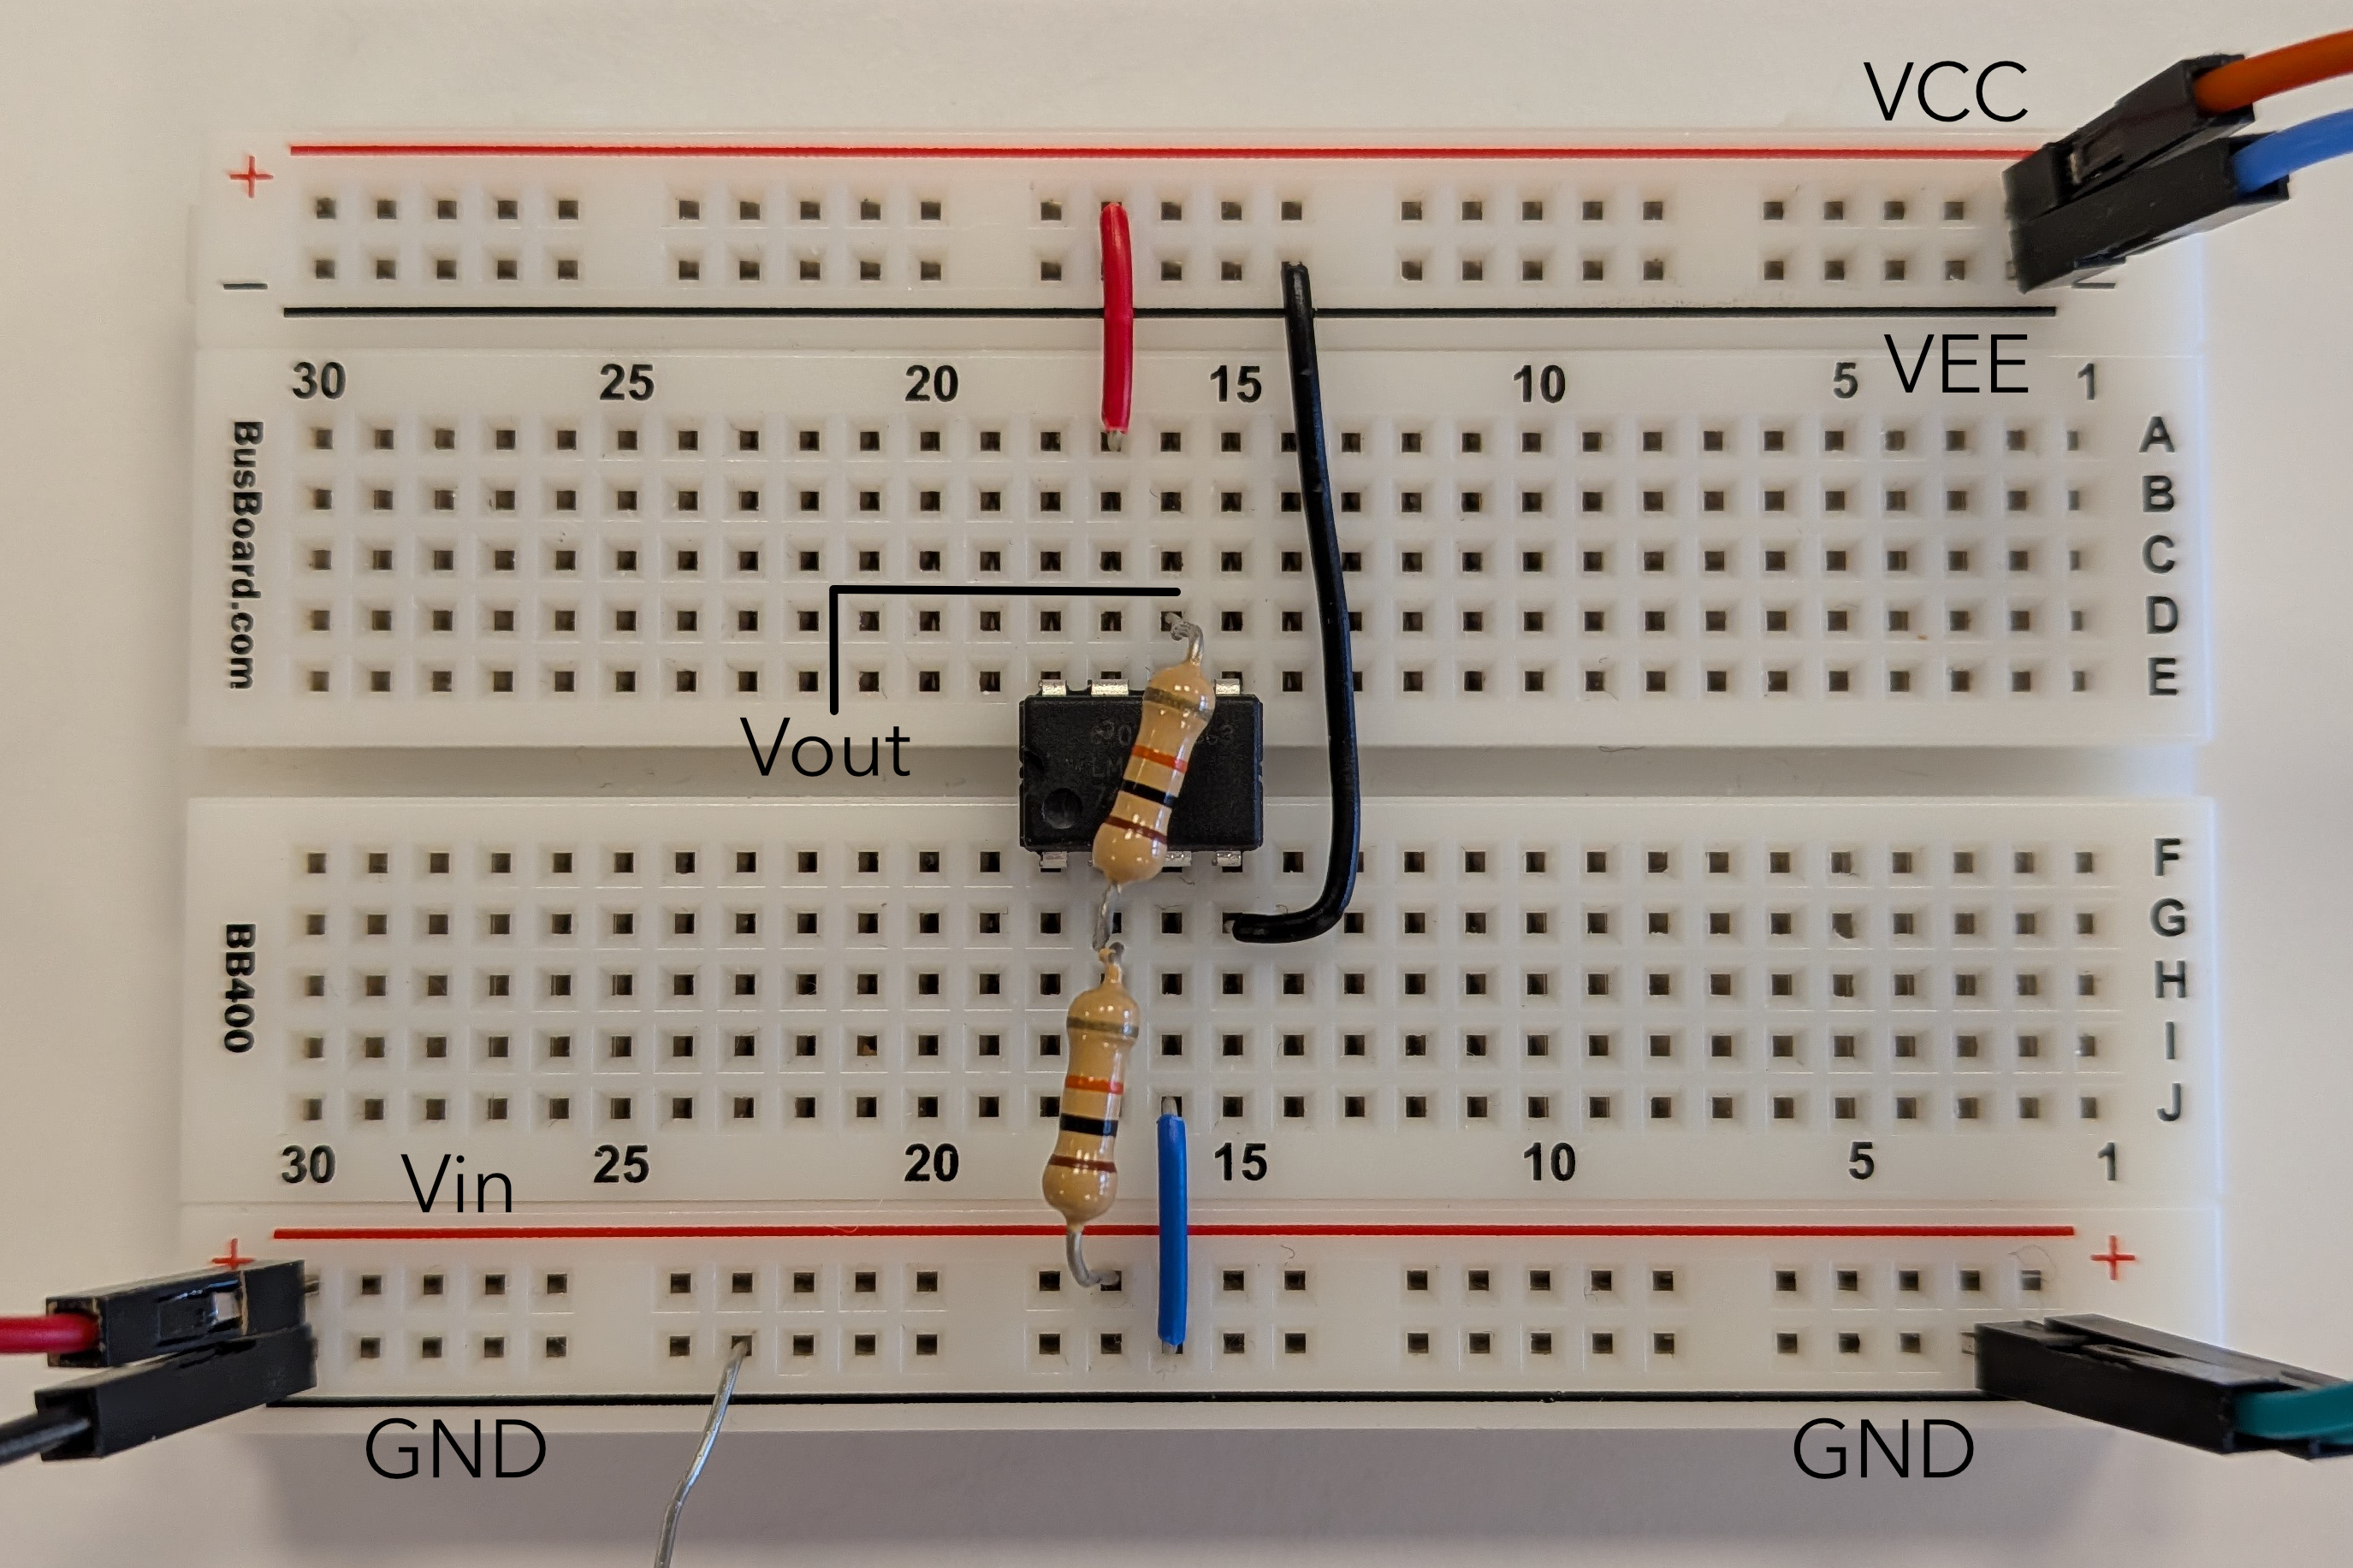
\includegraphics[width=\linewidth]{SlewCircuit.jpg}
\caption{Photograph of the amplifier circuit used for the slew rate measurement.}
\label{fig:Circuit1}
\end{figure}

%================  SINGLE FIGURE  =================================================%
\begin{figure}[!t]
\centering
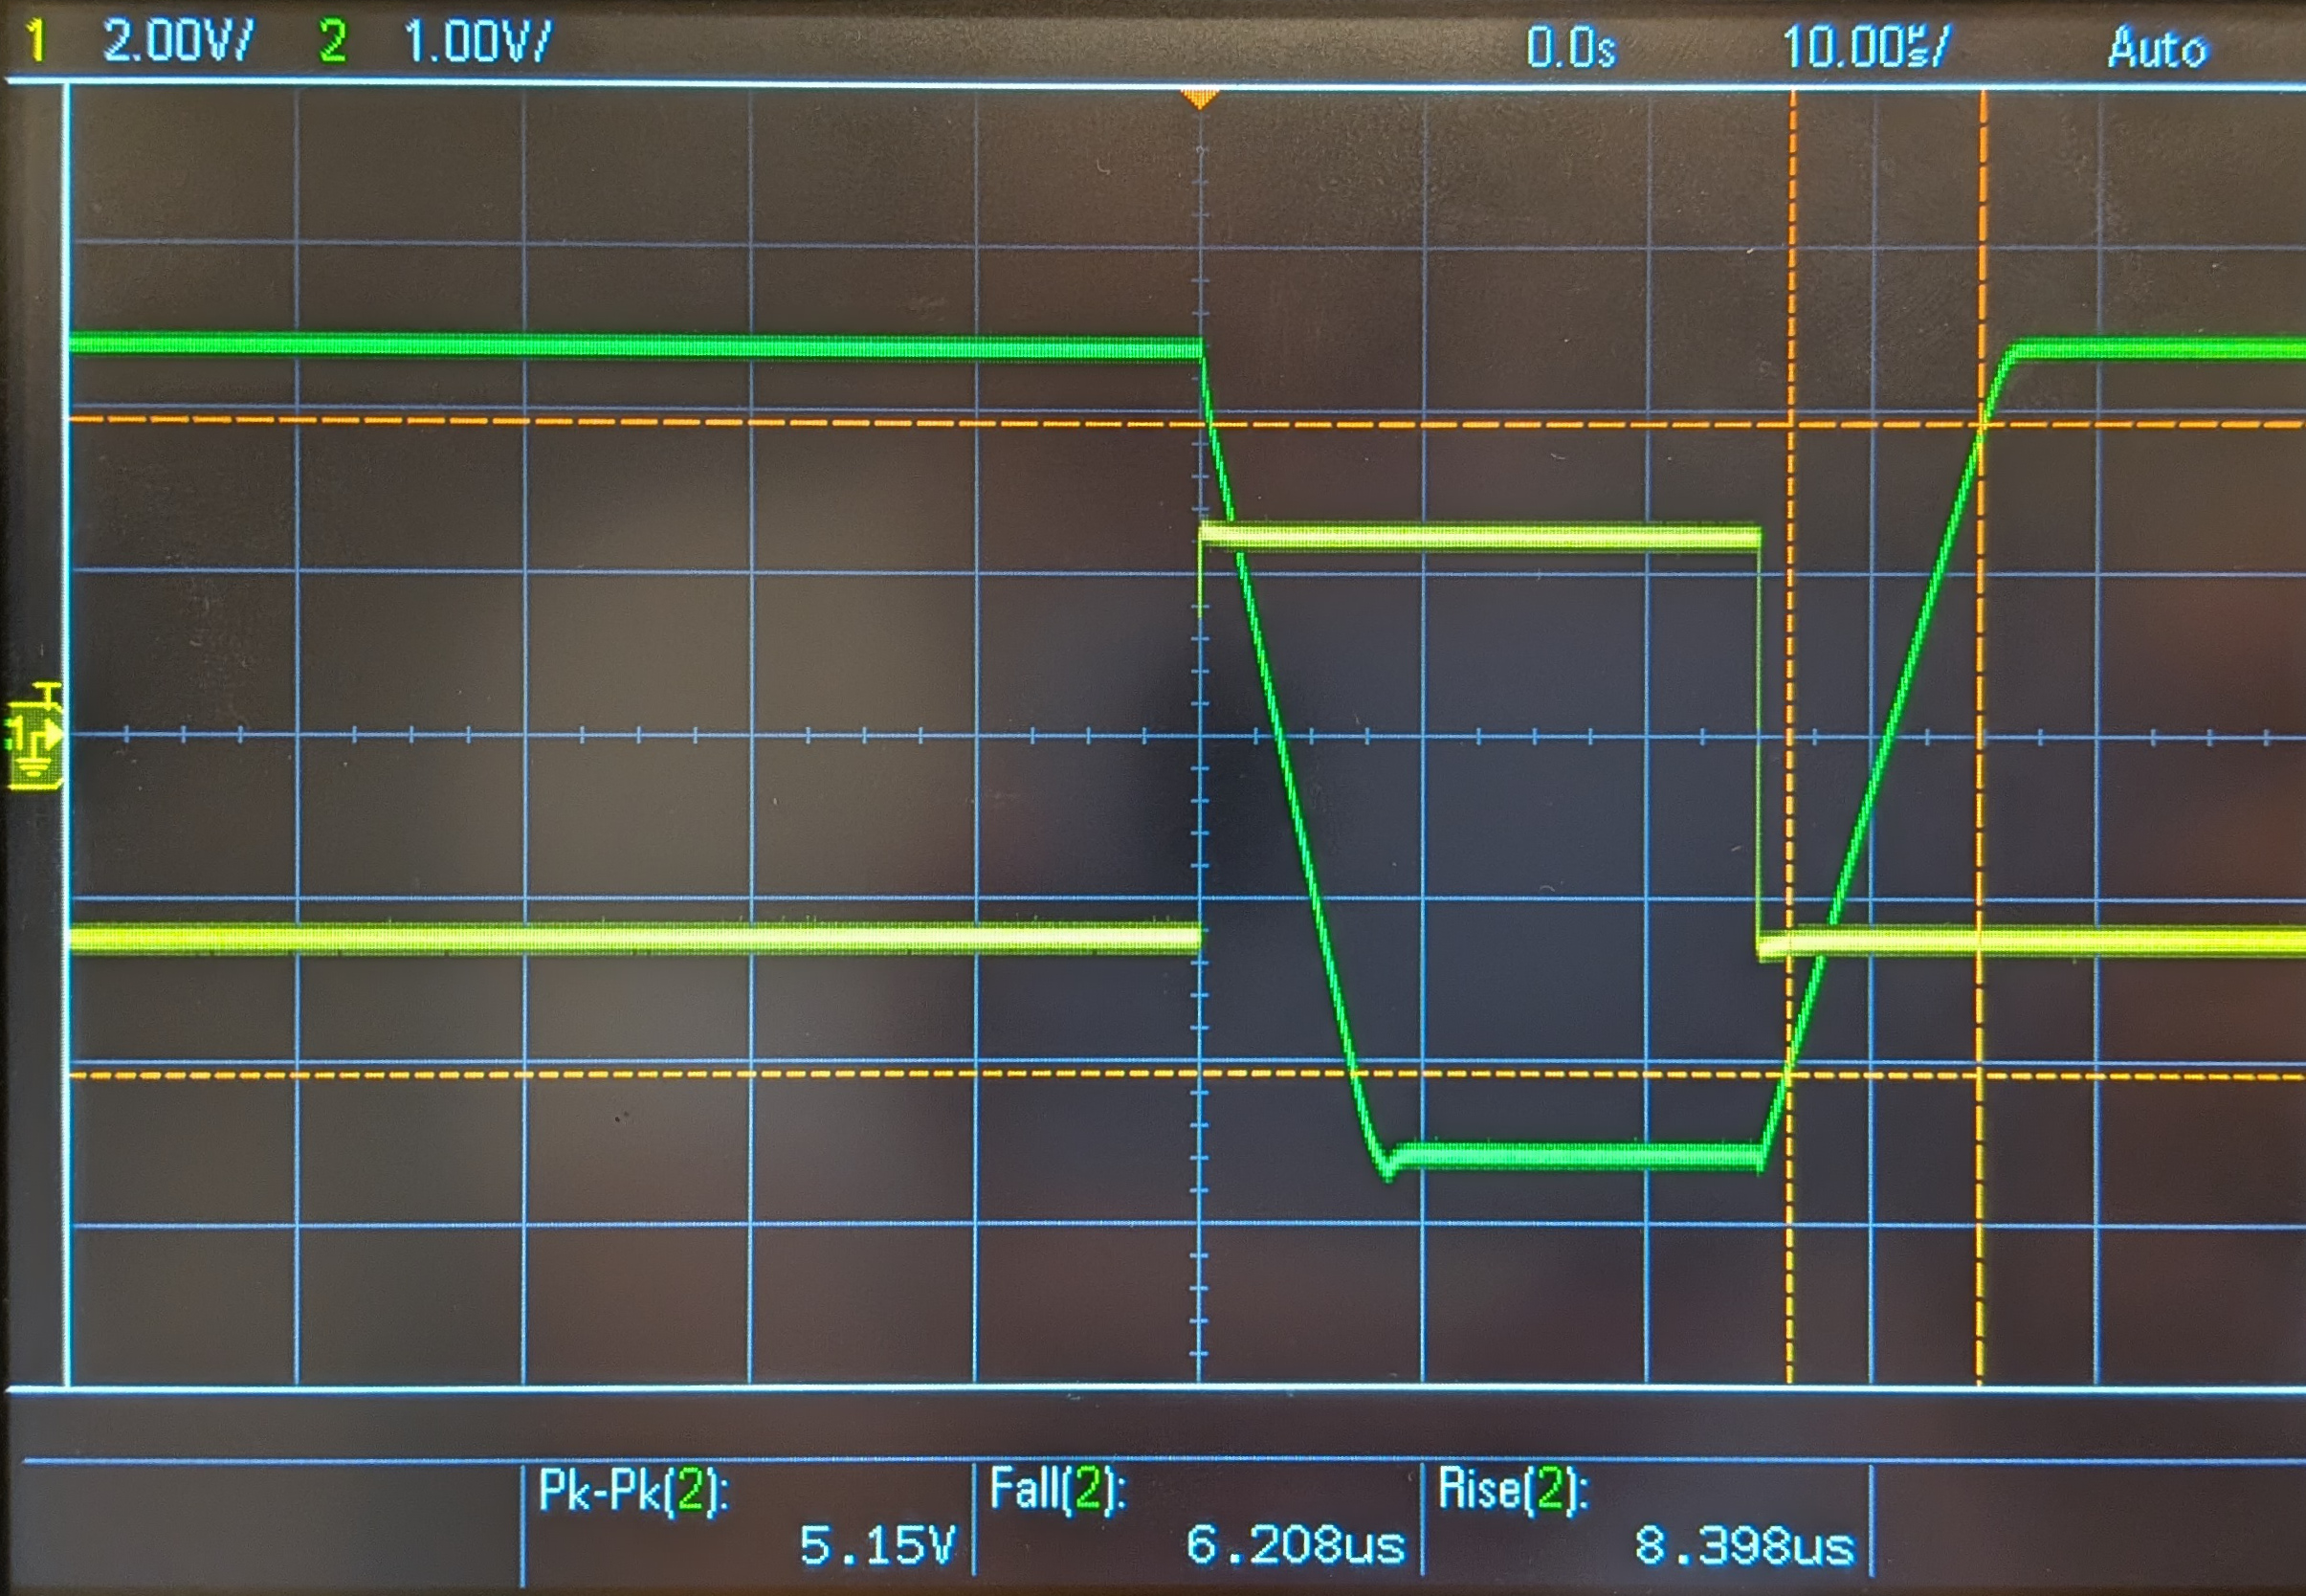
\includegraphics[width=\linewidth]{SlewRate.jpg}
\caption{Oscilloscope capture used to determine the slew rate.}
\label{fig:SlewRate}
\end{figure}

%================  EQUATION  ======================================================%
\begin{equation}
\label{eq:AvInv}
    \Ax{V(inv)} = - \frac{\Rx{f}}{\Rx{in}}
\end{equation}

%================  EQUATION  ======================================================%
\begin{equation}
\label{eq:SlewRate}
    \SRx{} = \frac{\Delta \Vx{out}}{\Delta t}
\end{equation}

% #endregion

%================  SUBSECTION  ====================================================%
\subsection{Determining CMRR}
% #region

The next step was to determine the common-mode rejection ratio of the operational amplifier.  
For this measurement the circuit was reconfigured as a differential amplifier with both inputs connected to the same signal-generator channel, ensuring identical signals at each input and creating a common-mode condition.  

A \(\qty{60}{\hertz}\) sine wave was applied to both inputs.  
The input and output voltages were observed on the oscilloscope, as shown in Figure~\ref{fig:CMRR}.  
From these measurements the voltage gain was calculated using (\ref{eq:Avdef}).  
Since the input signals were equal, this gain represents the common-mode gain, denoted \(\Ax{cm}\).  

The differential gain \(\Ax{dif}\) for the same configuration was estimated from the ideal resistor values using (\ref{eq:AvInv}), considering only the magnitude as phase inversion was not of interest.  
With both gains known, the common-mode rejection ratio was calculated using (\ref{eq:CMRR}).  

The CMRR was found to be \(\qty{74.4}{\decibel}\).  
This value is close to the typical specification of \(\qty{95}{\decibel}\) in the LM741 datasheet and within the expected range given that practical test conditions differ from those used for datasheet characterisation.  
In particular, the input resistance used here was \(\qty{100}{\ohm}\), whereas the datasheet specifies \(\Rx{in} \leq \qty{10}{\ohm}\), which likely explains the difference.  

Overall, the measurement shows that the LM741 provides good common-mode rejection under the given conditions, verifying the principle of differential signal amplification.  

%================  EQUATION  ======================================================%
\begin{equation}
\label{eq:Avdef}
    \Ax{V} = \frac{\Vx{out}}{\Vx{in}}
\end{equation}

%================  EQUATION  ======================================================%
\begin{equation}
\label{eq:CMRR}
    \CMRRx{dB} = 20 \log_{10}\!\left(\frac{\Ax{dif}}{\Ax{cm}}\right)
\end{equation}

%================  SINGLE FIGURE  =================================================%
\begin{figure}[!t]
\centering
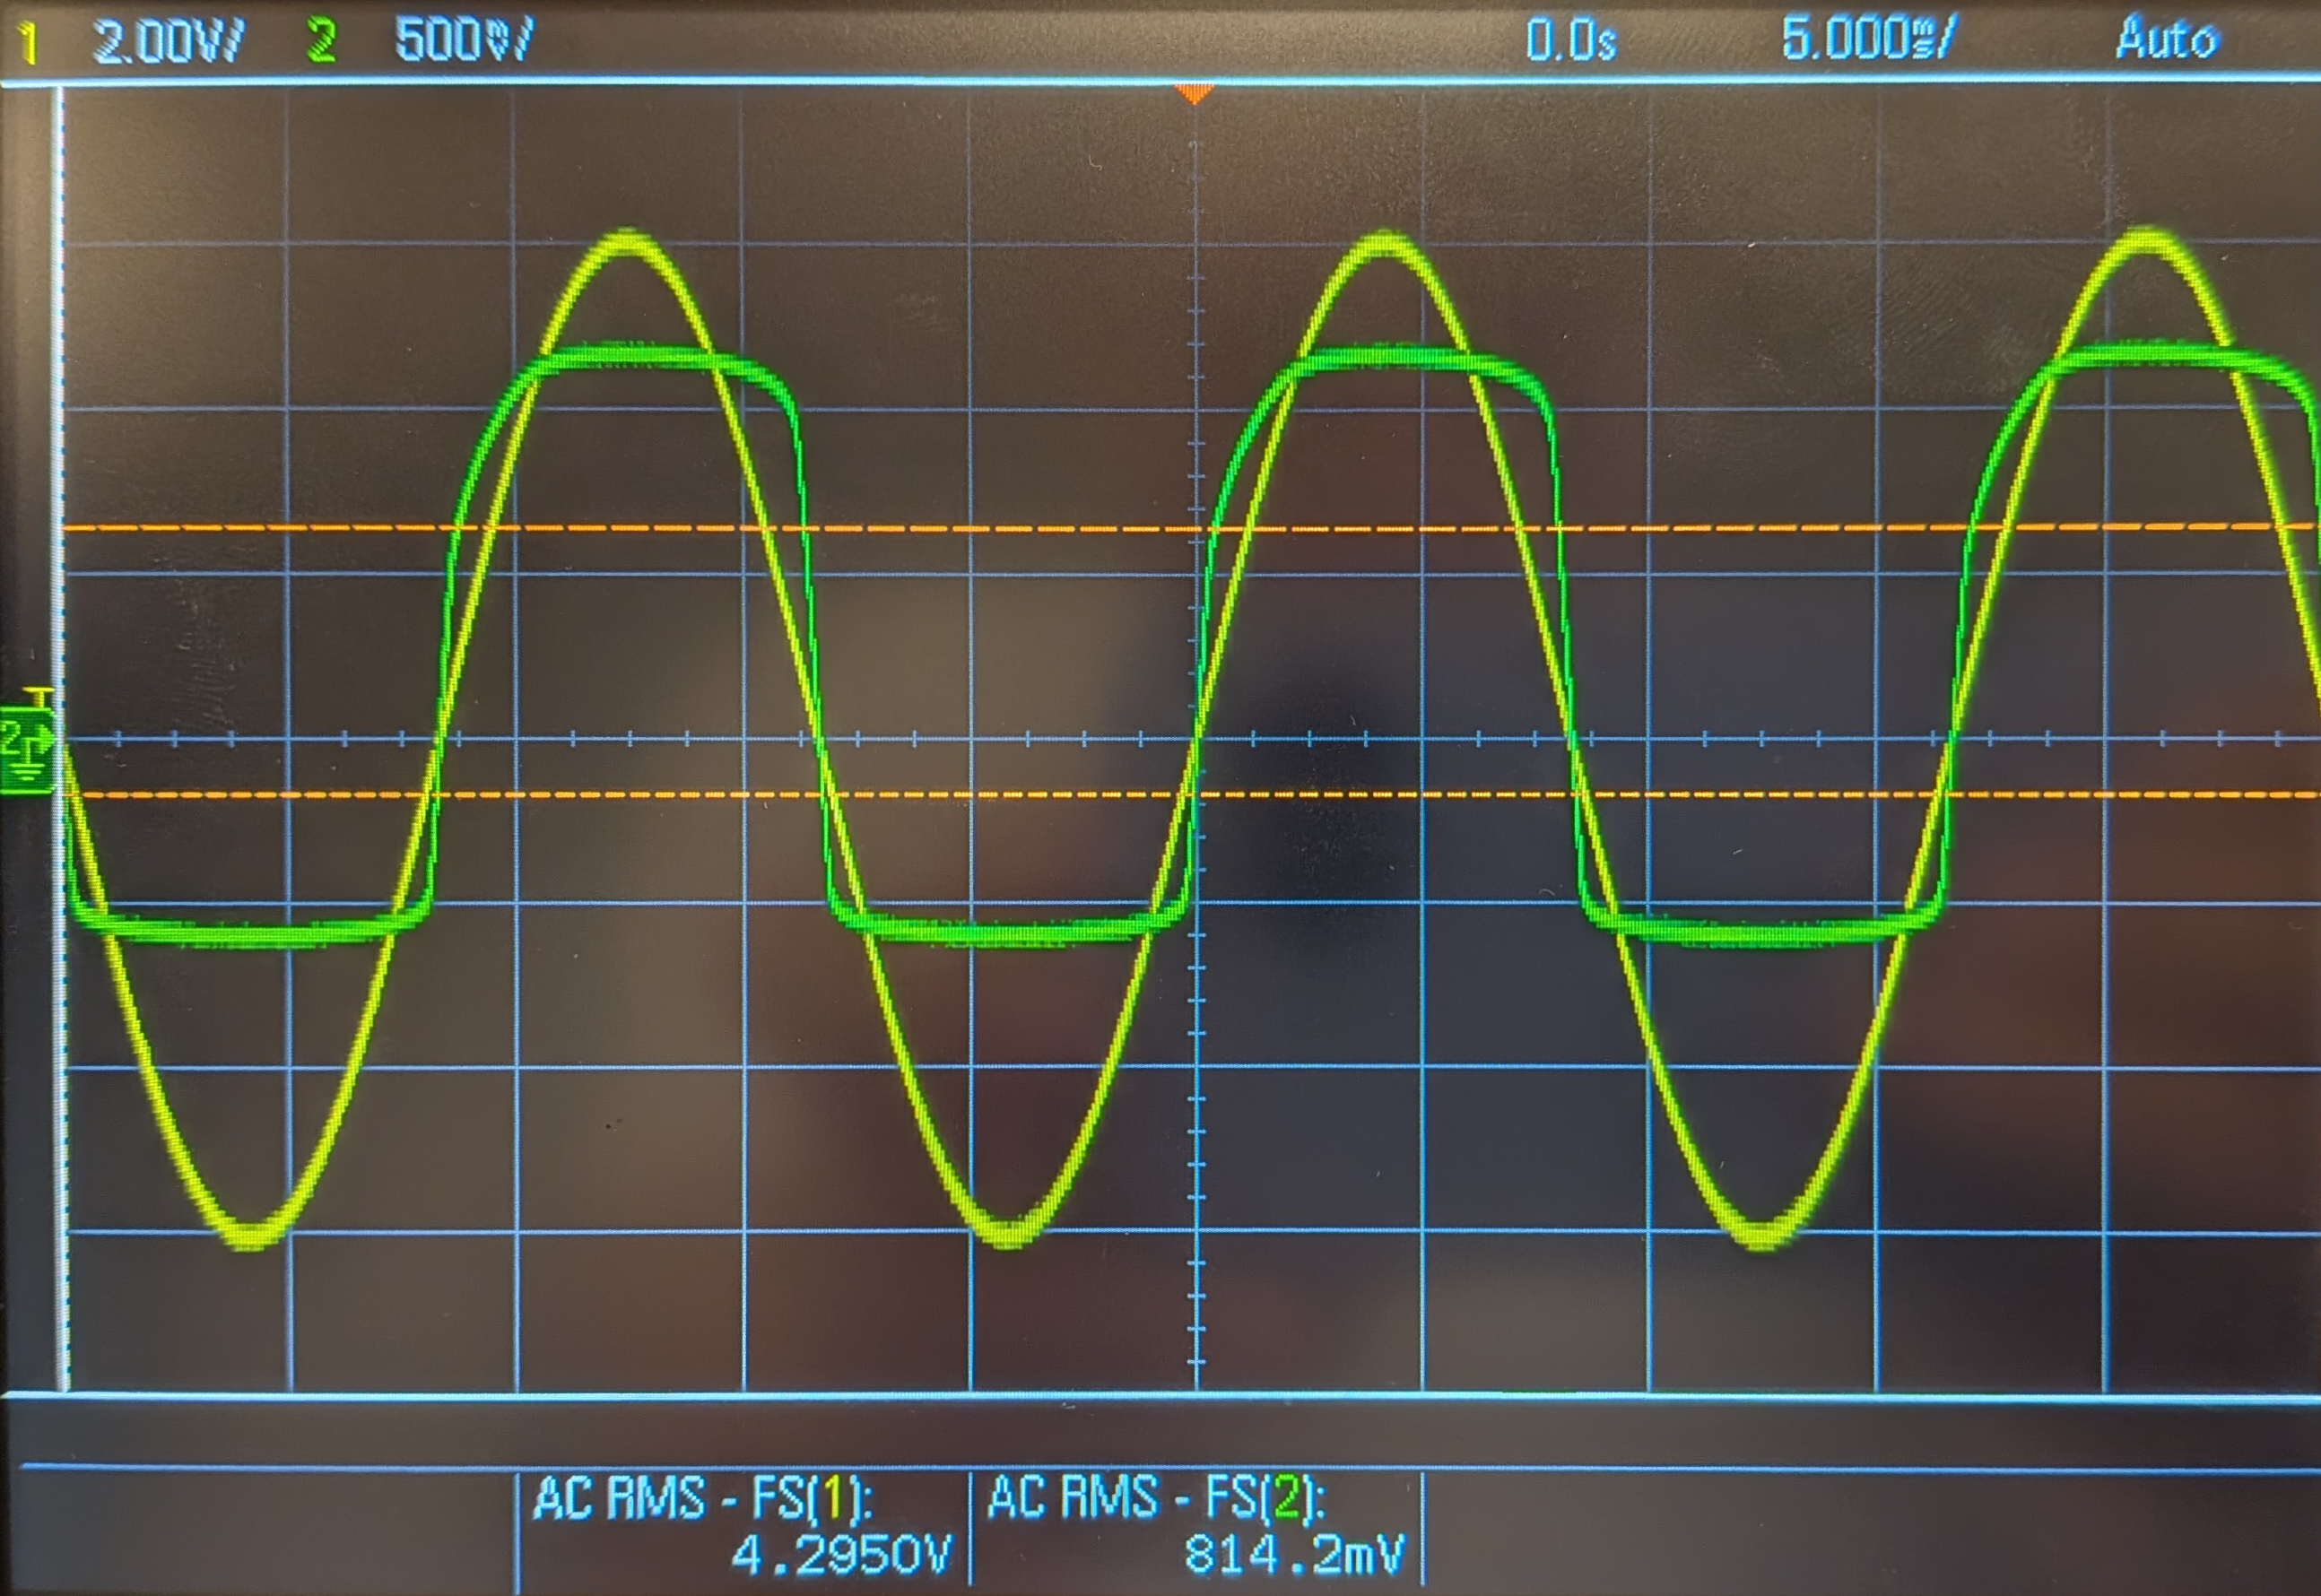
\includegraphics[width=\linewidth]{CMRR.jpg}
\caption{Oscilloscope capture used to determine the CMRR.}
\label{fig:CMRR}
\end{figure}


% #endregion

%================  SUBSECTION  ====================================================%
\subsection{Inverting amplifier}
% #region

An inverting amplifier circuit was constructed using the LM741 operational amplifier.  
The configuration employed a feedback resistor of \(\qty{100}{\kilo\ohm}\) and an input resistor of \(\qty{22}{\kilo\ohm}\).  
The theoretical voltage gain was calculated using (\ref{eq:AvInv}).  

A sine wave of \(\qty{10}{\kilo\hertz}\) was applied to the input, and both input and output voltages were measured using the oscilloscope.  
The measured voltage gain was then computed using (\ref{eq:Avdef}), including the negative sign to indicate phase inversion.  
Afterwards, the input resistor was replaced with a \(\qty{100}{\kilo\ohm}\) resistor, and the measurements were repeated to observe the effect of resistor ratio on voltage gain.  
All calculated and measured values are summarised in Table~\ref{tab:Inv}.  

The results show excellent agreement between theoretical and measured voltage gains, confirming the correct operation of the inverting amplifier configuration.  
Any small deviation is primarily due to component tolerances and measurement rounding.  

%================  TABLE  =========================================================%
\begin{table}[!b]
    \centering
    \caption{Inverting amplifier values}
    \label{tab:Inv}
    \begin{tabular}{l S[table-format=3.4] S[table-format=3.4] l}
        \toprule
        Parameter & {\(\Rx{in} = \qty{22}{\kilo\ohm}\)} & {\(\Rx{in} = \qty{100}{\kilo\ohm}\)} & Unit \\
        \midrule
        \(\Vx{in(measured)}\)      & 1.0074    & 1.0068      & \(\unit{\volt}\) \\
        \(\Vx{out(measured)}\)     & 4.508     & 1.0074      & \(\unit{\volt}\) \\
        \(\Ax{V(calculated)}\)     & -4.5455   & -1.0000     & --- \\
        \(\Ax{V(measured)}\)       & -4.4749   & -1.0006     & --- \\
        \bottomrule
    \end{tabular}
\end{table}

% #endregion

%================  SUBSECTION  ====================================================%
\subsection{Non-inverting amplifier}
% #region

A non-inverting amplifier circuit was constructed using the LM741 operational amplifier.  
The configuration employed a feedback resistor of \(\qty{100}{\kilo\ohm}\) and a resistor to ground of \(\qty{22}{\kilo\ohm}\), here denoted as \(\Rx{g}\).  
The theoretical voltage gain was calculated using (\ref{eq:AvNInv}).  

A sine wave of \(\qty{10}{\kilo\hertz}\) was applied to the input, and both input and output voltages were measured using the oscilloscope.  
The voltage gain was determined from the measured voltages using (\ref{eq:Avdef}).  
The same procedure was repeated after replacing the resistor to ground with a \(\qty{100}{\kilo\ohm}\) resistor to observe the effect of the resistor ratio on voltage gain.  
All results are summarised in Table~\ref{tab:NInv}.  

The measured voltage gains show excellent agreement with the theoretical values.  
As expected for the non-inverting configuration, the output signal maintains the same phase as the input while providing a positive voltage gain.  
Minor differences between theoretical and measured results are attributed to component tolerances and normal measurement uncertainty.  

%================  EQUATION  ======================================================%
\begin{figure}[t]
\begin{equation}
\label{eq:AvNInv}
    \Ax{V(ninv)} = 1 + \frac{\Rx{f}}{\Rx{g}}
\end{equation}
\vspace{-2em}
\end{figure}

%================  TABLE  =========================================================%
\begin{table}[!b]
    \centering
    \caption{Non-inverting amplifier values}
    \label{tab:NInv}
    \begin{tabular}{l S[table-format=3.4] S[table-format=3.4] l}
        \toprule
        Parameter & {\(\Rx{g} = \qty{22}{\kilo\ohm}\)} & {\(\Rx{g} = \qty{100}{\kilo\ohm}\)} & Unit \\
        \midrule
        \(\Vx{in(measured)}\)      & 1.0046  & 1.0073      & \(\unit{\volt}\) \\
        \(\Vx{out(measured)}\)     & 5.464   & 2.016       & \(\unit{\volt}\) \\
        \(\Ax{V(calculated)}\)     & 5.545   & 2.000       & --- \\
        \(\Ax{V(measured)}\)       & 5.439   & 2.001       & --- \\
        \bottomrule
    \end{tabular}
\end{table}

% #endregion

%================  SUBSECTION  ====================================================%
\subsection{Unity gain follower}
% #region

A unity gain follower circuit was constructed using the LM741 operational amplifier.  
This configuration directly connects the output to the inverting input, providing a voltage gain of one.  
As no resistors are used, the circuit simply buffers the input signal without amplification or inversion.  

A sine wave of \(\qty{10}{\kilo\hertz}\) was applied to the input, and both input and output voltages were measured using the oscilloscope.  
The voltage gain was then calculated using (\ref{eq:Avdef}).  
All measured and calculated values are summarised in Table~\ref{tab:Unity}.  

The measured gain closely matches the theoretical value of unity, confirming that the LM741 operates correctly as a voltage follower under the given test conditions.  

%================  TABLE  =========================================================%
\begin{table}[!b]
    \centering
    \caption{Unity gain amplifier values}
    \label{tab:Unity}
    \begin{tabular}{l S[table-format=3.4] l}
        \toprule
        Parameter & {Value} & Unit \\
        \midrule
        \(\Vx{in(measured)}\)       & 2.0119    & \(\unit{\volt}\) \\
        \(\Vx{out(measured)}\)      & 2.0116    & \(\unit{\volt}\) \\
        \(\Ax{V(calculated)}\)      & 1.0000    & --- \\
        \(\Ax{V(measured)}\)        & 0.9999    & --- \\
        \bottomrule
    \end{tabular}
\end{table}

% #endregion

%================  SUBSECTION  ====================================================%
\subsection{Summing amplifier}
% #region

A summing amplifier circuit was constructed using the LM741 operational amplifier.  
In the first configuration, a weighted summing amplifier was implemented with a feedback resistor of \(\qty{100}{\kilo\ohm}\), and two input resistors of \(\qty{100}{\kilo\ohm}\) and \(\qty{22}{\kilo\ohm}\) for channels one and two, respectively.  
Each input signal was a \(\qty{1}{\volt}\) sine wave, and both inputs were connected to the same output channel of the signal generator to ensure identical phase and amplitude.  
The theoretical output voltage was calculated using (\ref{eq:Vosum}).  

The input and output waveforms were observed on the oscilloscope, as shown in Figure~\ref{fig:WeightedSum}.  
The measured output voltage was then compared to the calculated value to verify the theoretical prediction.  

After completing the weighted measurement, the \(\qty{22}{\kilo\ohm}\) input resistor was replaced with another \(\qty{100}{\kilo\ohm}\) resistor, creating a balanced summing amplifier.  
A photograph of this configuration is shown in Figure~\ref{fig:Sum}.  
The same procedure was repeated, and the measured output voltage was compared with the calculated value.  
All results are summarised in Table~\ref{tab:Sum}.  

The results show that both configurations behaved as expected, with measured output voltages in close agreement with theoretical calculations.  
Small differences are mainly due to resistor tolerances, as the measured resistor values produced results that closely matched the measured output when used in the theoretical calculations.  
This confirms that the LM741 performs accurately as a linear summing amplifier, capable of producing both weighted and balanced signal combinations.  

%================  EQUATION  ======================================================%
\begin{figure}[t]
\begin{equation}
\label{eq:Vosum}
    \Vx{out} = \Vx{in1} \frac{\Rx{f}}{\Rx{in1}} + \Vx{in2} \frac{\Rx{f}}{\Rx{in2}}
\end{equation}
\vspace{-2em}
\end{figure}

%================  SINGLE FIGURE  =================================================%
\begin{figure}[!b]
\centering
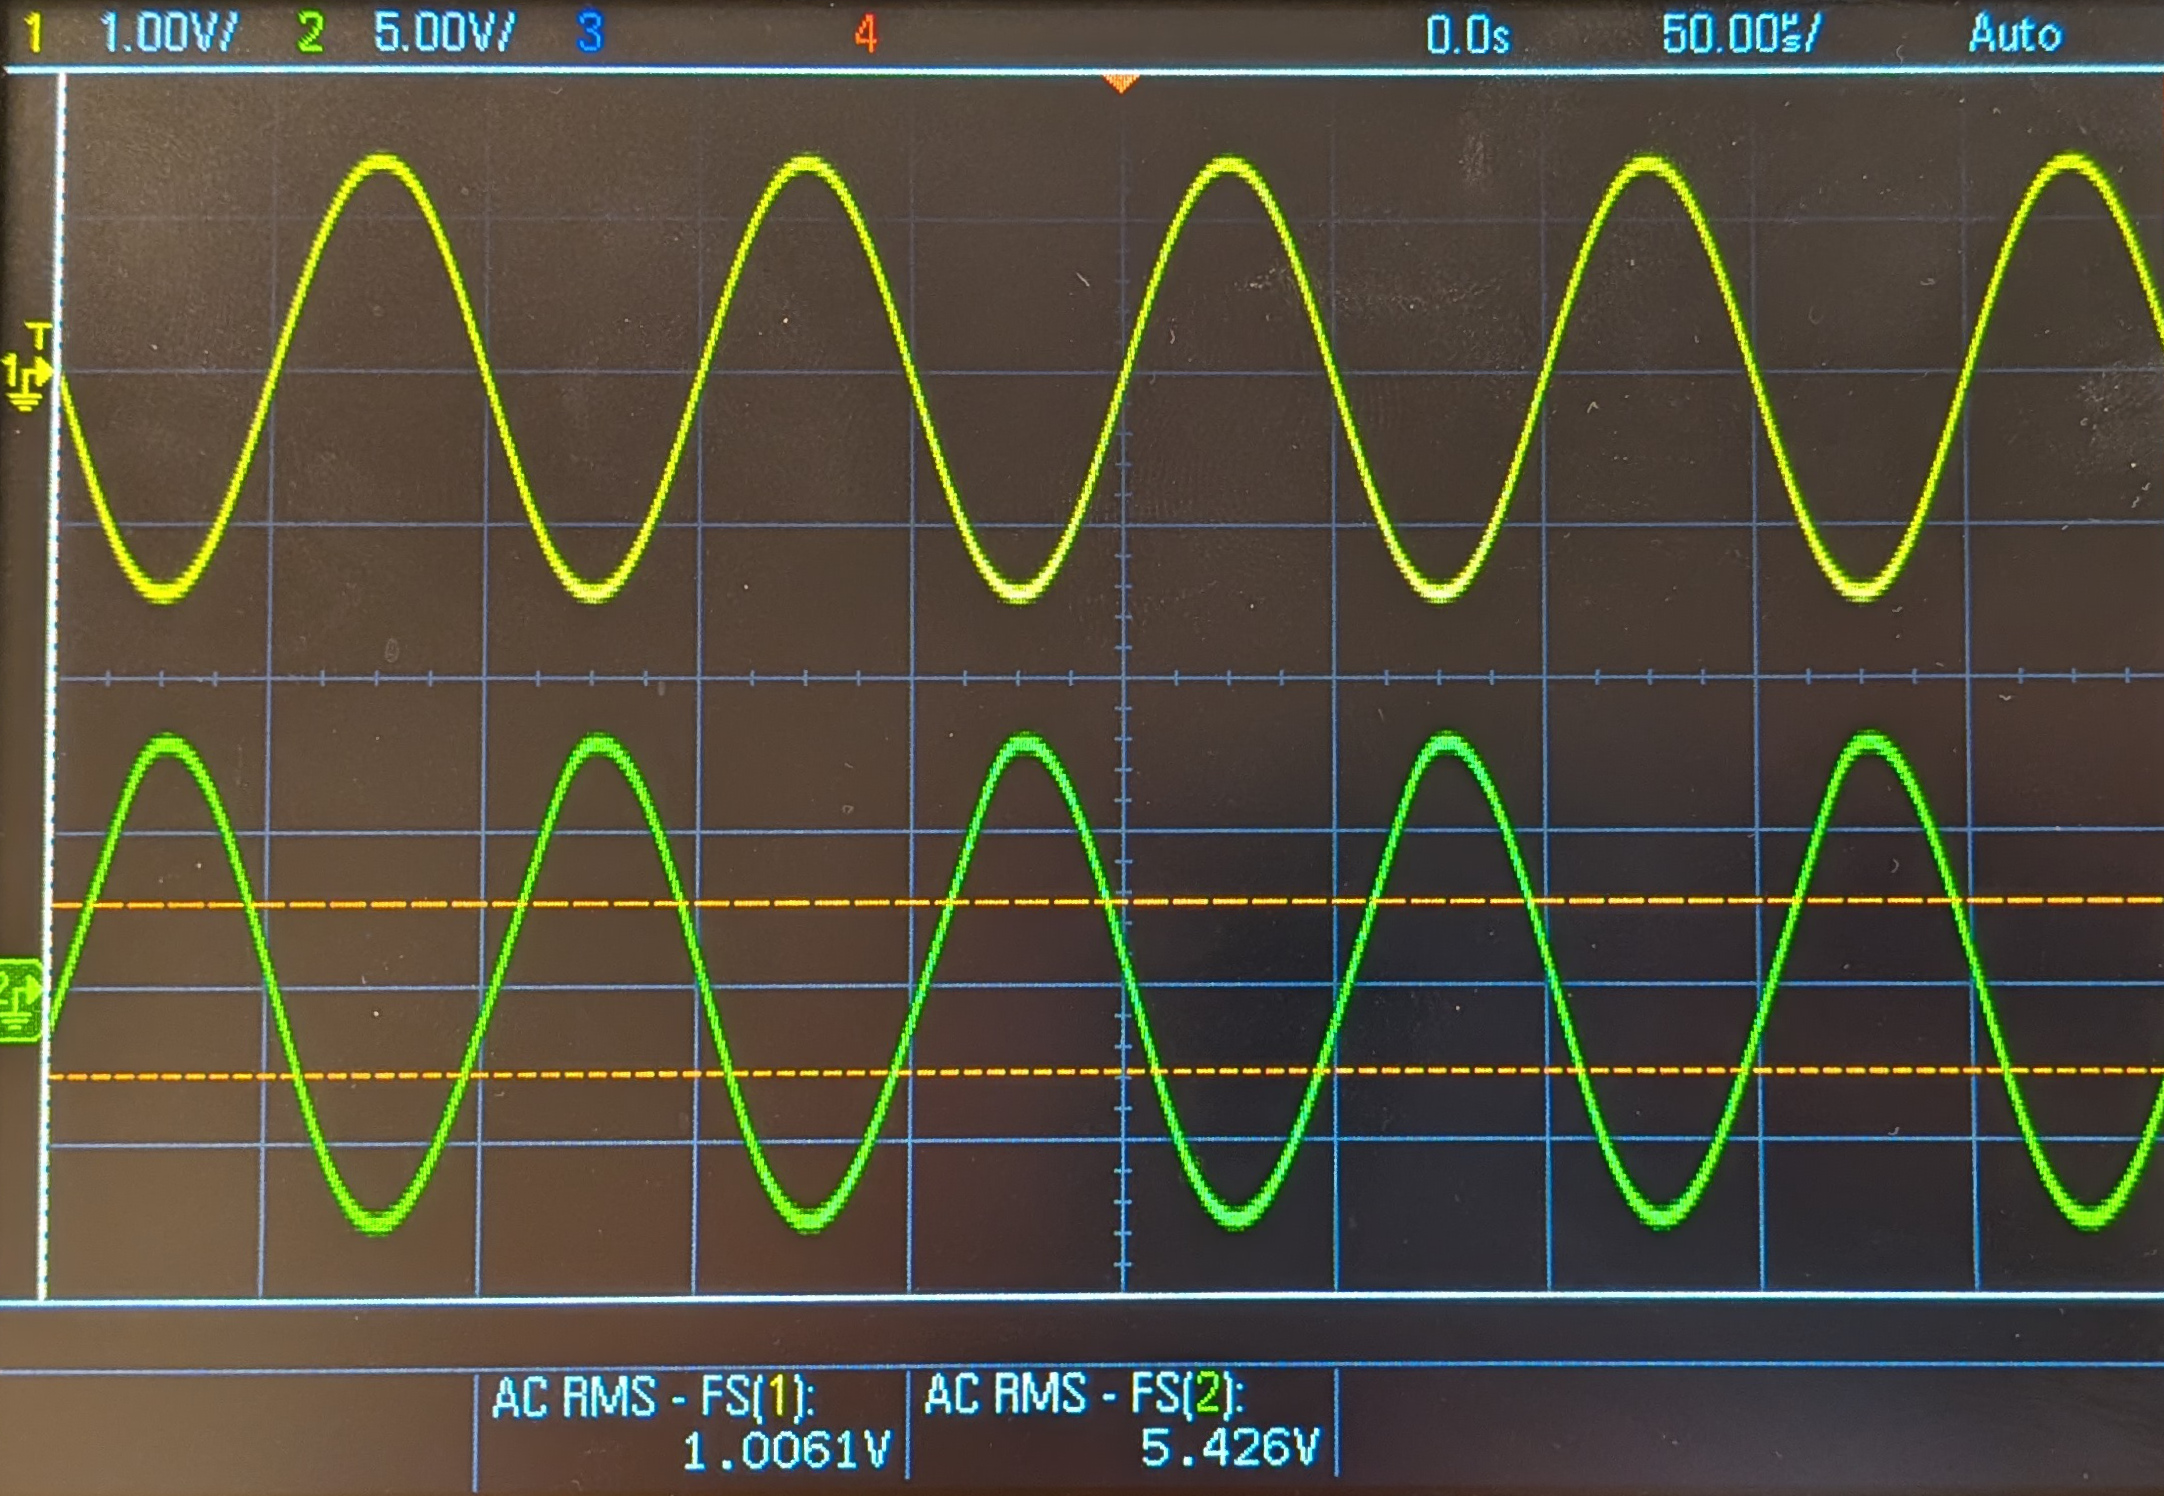
\includegraphics[width=\linewidth]{WeightedSum.jpg}
\caption{Oscilloscope capture showing the weighted summing amplifier output.}
\label{fig:WeightedSum}
\end{figure}

%================  SINGLE FIGURE  =================================================%
\begin{figure}[!b]
\centering
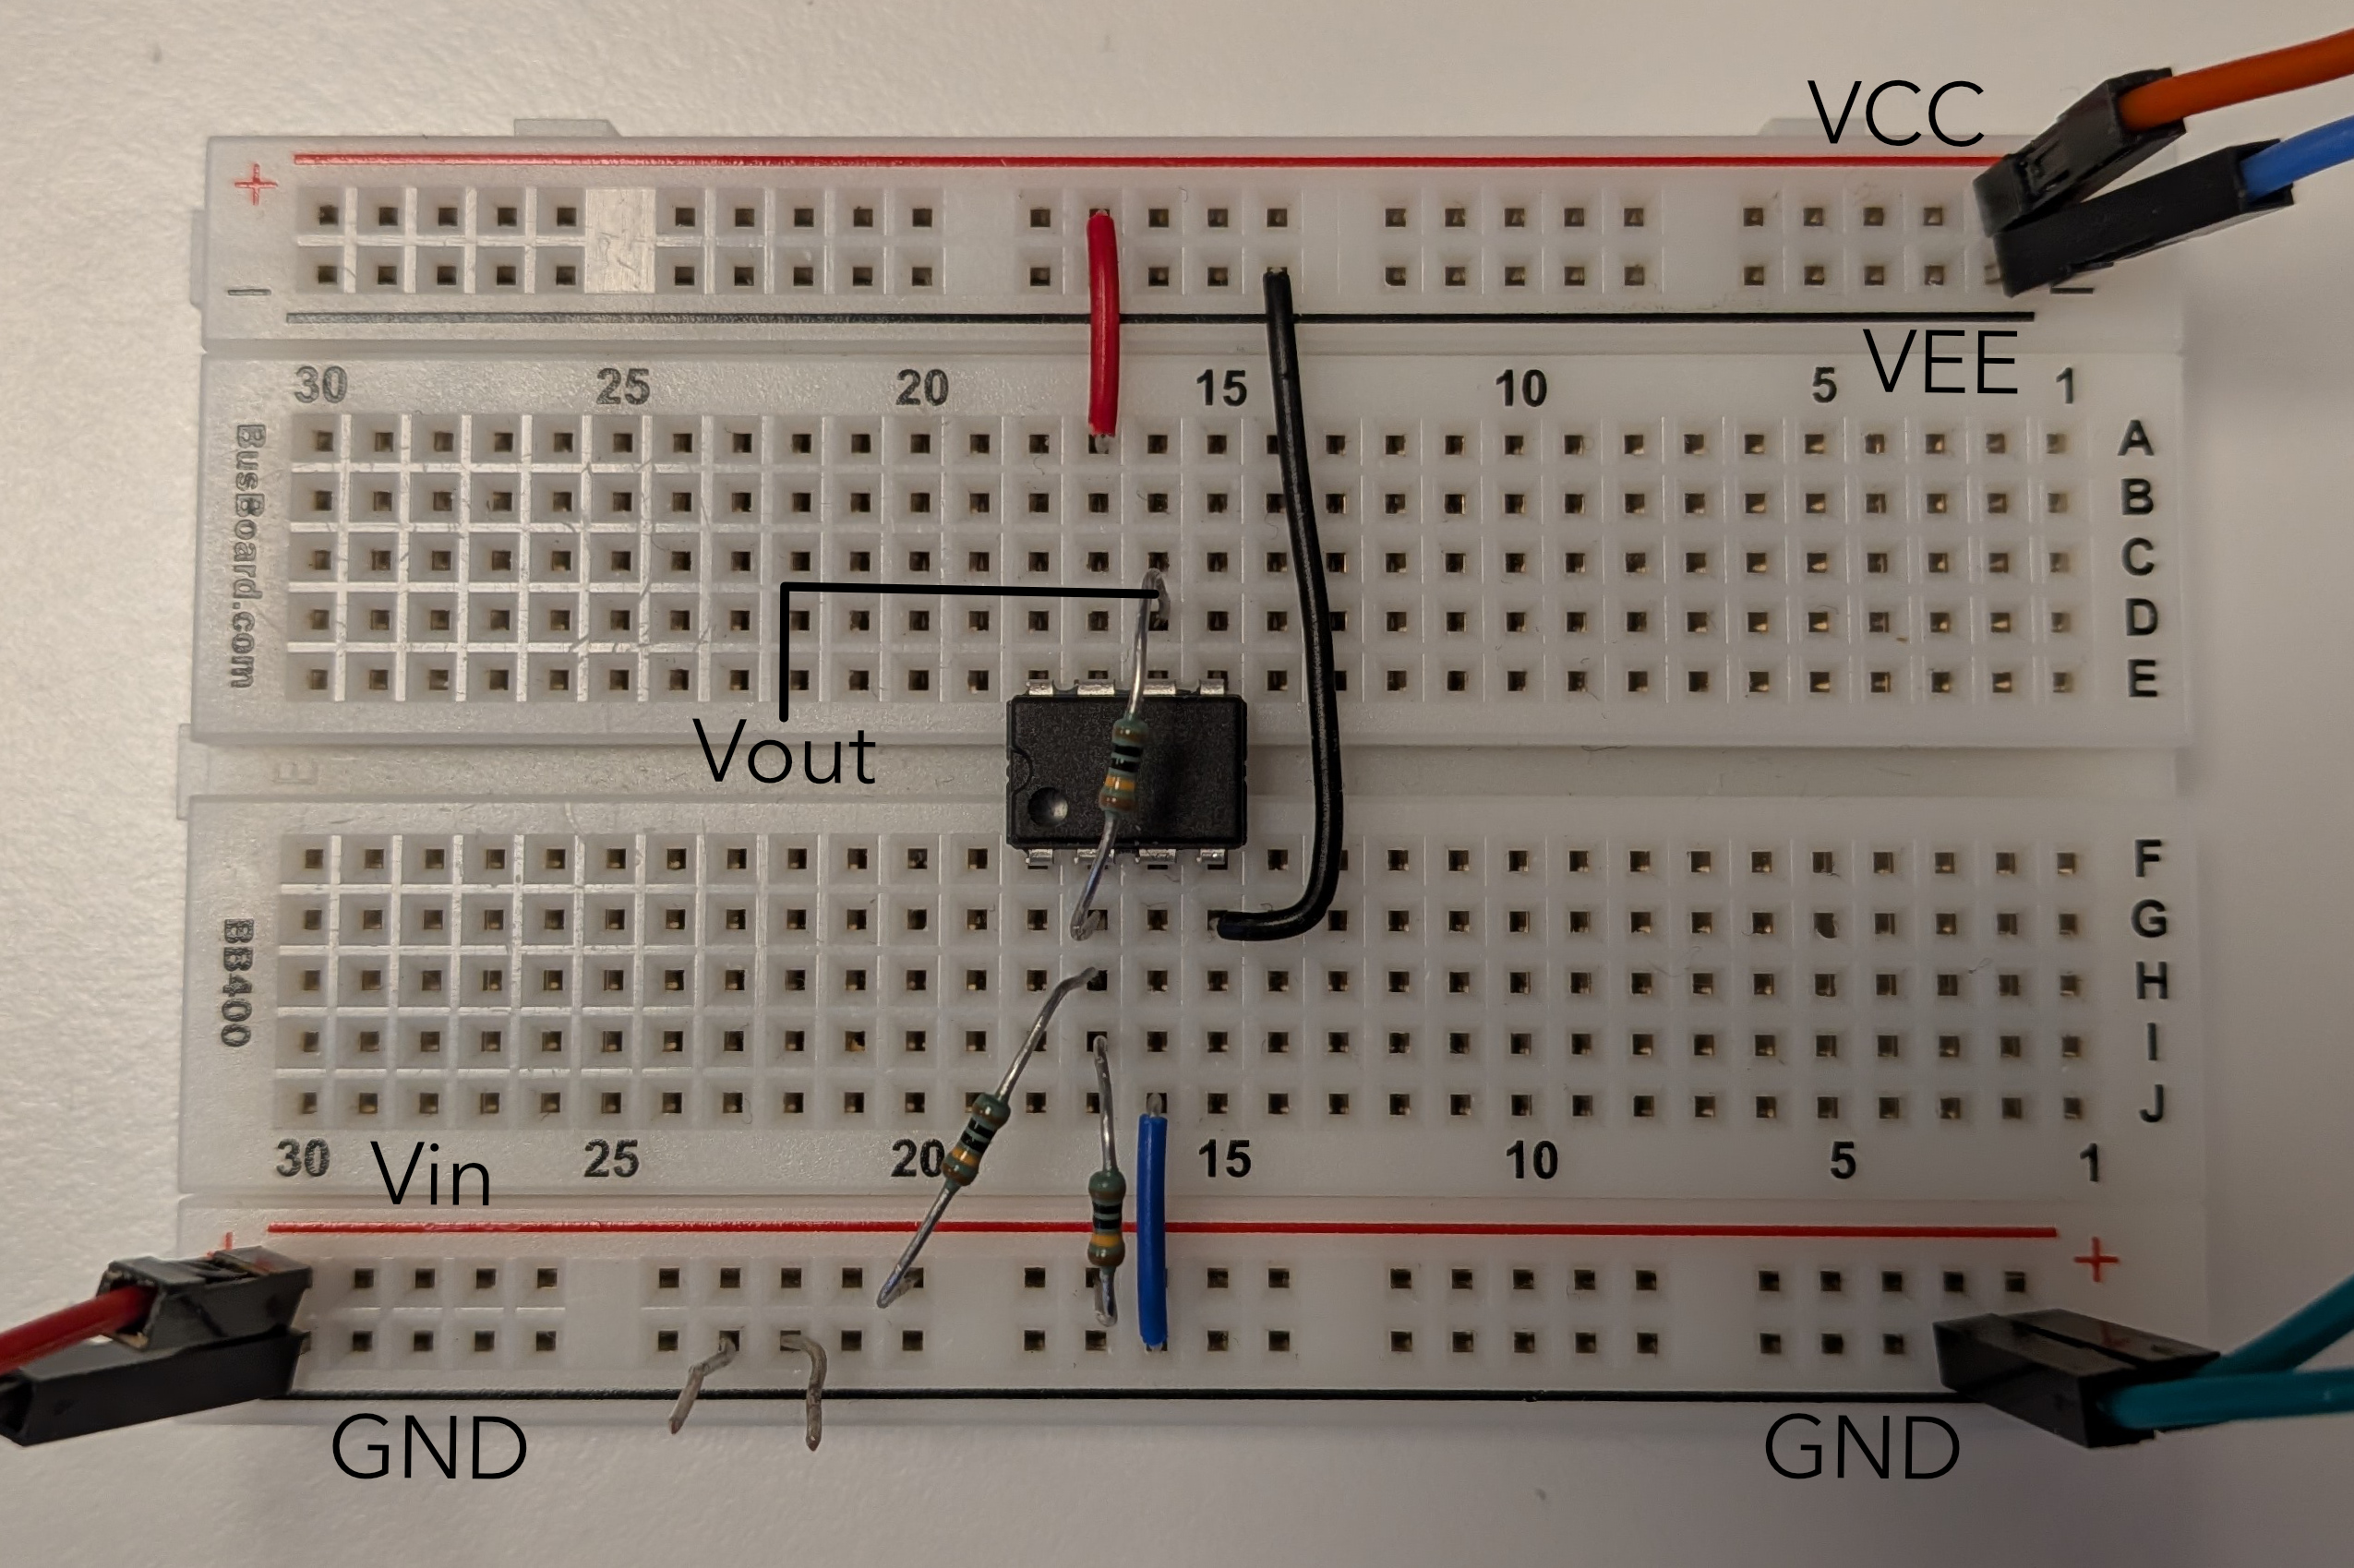
\includegraphics[width=\linewidth]{SumCircuit.jpg}
\caption{Photograph of the summing amplifier circuit.}
\label{fig:Sum}
\end{figure}



%================  TABLE  =========================================================%
\begin{table}[!t]
    \centering
    \caption{Summing amplifier values}
    \label{tab:Sum}
    \begin{tabular}{l S[table-format=3.4] S[table-format=3.4] l}
        \toprule
        Parameter & {\(\Rx{in2} = \qty{22}{\kilo\ohm}\)} & {\(\Rx{in2} = \qty{100}{\kilo\ohm}\)} & Unit \\
        \midrule
        \(\Vx{in(calculated)}\)     & 1.0000  & 1.0000       & \(\unit{\volt}\) \\
        \(\Vx{in(measured)}\)       & 1.0061  & 1.0079       & \(\unit{\volt}\) \\
        \(\Vx{out(calculated)}\)    & 5.545   & 2.0000       & \(\unit{\volt}\) \\
        \(\Vx{out(measured)}\)      & 5.426   & 2.0113       & \(\unit{\volt}\) \\
        \bottomrule
    \end{tabular}
\end{table}

% #endregion

%================  CONCLUSION  ====================================================%
\section{Conclusion}
% #region

This laboratory exercise investigated several fundamental characteristics and configurations of the LM741 operational amplifier.  
The slew rate, common-mode rejection ratio, and voltage gains of multiple amplifier configurations were measured and compared with theoretical expectations.  

The measured slew rate was \(\qty{0.83}{\volt\per\micro\second}\) for the rising edge and \(\qty{0.61}{\volt\per\micro\second}\) for the falling edge, which agrees closely with the typical specification of the device.  
The CMRR was determined to be approximately \(\qty{74.4}{\decibel}\), which is reasonable when considering the simplified test setup and higher input resistance used compared with the datasheet test conditions.  

\newpage

Both the inverting and non-inverting amplifier circuits exhibited the expected voltage gains, with measured results closely matching theoretical calculations.  
The unity gain follower performed as expected, providing an output voltage effectively identical to the input.  
Finally, the summing amplifier correctly demonstrated both weighted and balanced addition of input signals, with only small deviations from calculated values explained by resistor tolerances.  

Overall, the LM741 operational amplifier demonstrated consistent and predictable behaviour in all tested configurations.  
The experimental results validate the theoretical models of op-amp operation and confirm the practical accuracy of the LM741 for general analogue circuit applications.  

% #endregion


%================  ACKNOWLEDGMENT  ================================================%
\section*{Acknowledgment}
% #region
This report corresponds to Lab~06 in the course \emph{Elektroniske enheter og kretser}.
All related materials (\LaTeX~sources, raw data, figures, codes and more) are released under the MIT License and available at \url{https://github.com/Kjelseth/EEK_lab}.
% #endregion

\end{document}